The \textit{users} module is responsible for maintaining demographic information
about the registered users of the system, including the Autority levels of each
user.

\subsection{Scope}
The scope for the users module is shown in Figure \ref{Users Scope}
\begin{figure}[H]
  \begin{center}
  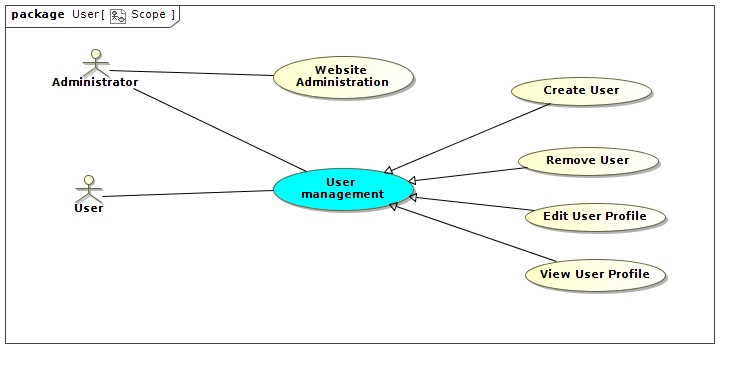
\includegraphics[scale=0.5]{../Diagrams and Charts/Users/Scope.jpg}
  \caption{Users Scope}
  \end{center}
  \label{Users Scope}
\end{figure}
The scope of the users module include:
\begin{itemize}
	\item The Super User can add and remove Administrator users
	\item Administrator users can add and remove Regular Users
	\item Any person who wants use the bechmarking service can add their
	profiles to the system and become a user. They can then also edit or
	remove their profiles
	\item Any user can view the profile of any Administrator or Regular
	user
\end{itemize}

\subsection{Domain Model}
The domain model for the users module is shown in Figure \ref{Users Domain Model}
\begin{figure}[H]
  \begin{center}
  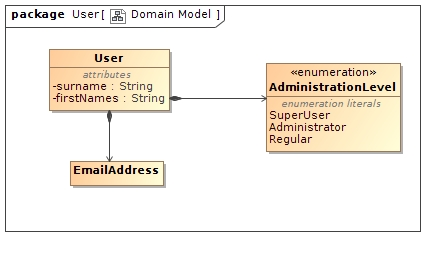
\includegraphics[scale=1.0]{../Diagrams and Charts/Users/Domain Model.jpg}  
  \caption{Users Domain Model}
  \end{center}
  \label{Users Domain Model}
\end{figure}
For each user a Surname, First Names and Email Address will be stored.
There are 3 main types of users who
are at different authority levels. There is one and only one "Super User" who
will have full authority over the entire system. Then there are "Administrator"
users who can be assigned or removed by the Super User. The main function of
the Super User is to manage the Administrator users. The Administrator user
wil have the permissions needed to manage the website and to add or remove.
Regular Users if nessesary. Lastly the "Regular Users"
can be created by anyone who wants to use the benchmarking service. These users
will be able to use the service but not do anything administrative.
